\documentclass[aps,prd,onecolumn,nofootinbib,preprint]{revtex4-2}

\usepackage{amsmath,amssymb,amsfonts}
\usepackage{graphicx}
\usepackage{hyperref}

\begin{document}

\title{From Mutual-Information Laplacians to Cosmological Dynamics:\\
An Effective Stress--Energy Tensor from an Assumed Entanglement-Decay Ansatz}

\author{Paul Jarvis}
\email{mrpaulwjarvis@gmail.com}
\affiliation{Independent Researcher, United Kingdom}

\date{\today}

\begin{abstract}
We work out the macroscopic stress--energy tensor implied by a specific ansatz for a pre-geometric
quantum substrate: that mutual information between subregions decays with relational distance as a
power law, $I(i,j) \sim d(i,j)^{-\alpha}$. Beginning with a canonical partition function over the
nonzero eigenmodes of the resulting mutual-information (MI) Laplacian, we show that this ansatz
alone -- combined with the elementary homogeneity of a power-law kernel -- fixes how the Laplacian
spectrum scales under a global rescaling of distances, exactly and at any system size. Matching
that scaling to the standard cosmological continuity equation yields an equation-of-state
dictionary, $w_{\mathrm{eff}} = \alpha/3 - 1$, where $\alpha$ is the assumed entanglement decay exponent.
Under this ansatz, the de Sitter phase appears as the $\alpha \to 0$ limit, where relational
connectivity becomes distance-independent and the emergent cosmic fluid locks to
$w_{\mathrm{eff}} = -1$, without invoking vacuum energy or scalar fields. The resulting mapping
$T^{\mathrm{eff}}_{\mu\nu}(\mathcal{L}_{\mathrm{MI}})$ is an exact algebraic consequence of the assumed kernel
form; justifying that form physically, rather than the algebra connecting it to the equation of
state, is the open problem this framework leaves for future work.
\end{abstract}

\maketitle

\section{Introduction}

A central challenge in emergent-gravity and quantum-information approaches to spacetime is
connecting microscopic relational data to macroscopic cosmological dynamics. While numerous
frameworks demonstrate how geometric notions may arise from entanglement patterns, far fewer work
out an explicit effective stress--energy tensor that sources the Einstein equations. The present
work does so under a specific, stated ansatz: that mutual information decays with relational
distance as a power law. Given that ansatz, $T_{\mu\nu}^{\mathrm{eff}}$ follows directly from the spectral
properties of the resulting mutual-information (MI) Laplacian defined on a pre-geometric quantum
substrate.

The argument is self-contained and independent of any specific microscopic Hamiltonian once the
ansatz is granted. It relies on three structural ingredients: (i) the MI--Laplacian spectrum, (ii) a
canonical partition function over its nonzero eigenmodes, and (iii) the exact homogeneous scaling
of Laplacian eigenvalues under global spatial expansion that follows algebraically from the
power-law ansatz. These elements are sufficient to determine the emergent energy density, pressure,
and equation of state of the macroscopic cosmic fluid, conditional on the ansatz holding.

\section{Relational substrate and MI--Laplacian}

Consider a quantum many-body system partitioned into subregions labelled by indices $i,j$. The
mutual information between two subregions is
\begin{equation}
I(i,j) = S(\rho_i) + S(\rho_j) - S(\rho_{ij}),
\end{equation}
where $S(\rho)$ is the von Neumann entropy. The matrix $I(i,j)$ serves as a relational measure of
proximity: highly entangled regions are ``close'' in the emergent geometry.

From the normalized mutual-information matrix we construct a symmetric adjacency matrix
$A_{ij}$ and the corresponding combinatorial Laplacian,
\begin{equation}
L_{\mathrm{MI}} = D - A,
\end{equation}
where $D_{ii} = \sum_j A_{ij}$. Let the eigenvalues of $L_{\mathrm{MI}}$ be
\begin{equation}
0 = \lambda_0 < \lambda_1 \le \cdots \le \lambda_{N-1}.
\end{equation}
These eigenvalues encode the stiffness of relational degrees of freedom and constitute the
fundamental microscopic spectrum of the substrate.

\section{Canonical partition function}

We define a canonical partition function over the nonzero eigenmodes:
\begin{equation}
Z(\beta) = \sum_{n=1}^{N-1} e^{-\beta \lambda_n},
\end{equation}
where $\beta$ is an inverse entanglement temperature. The internal energy is
\begin{equation}
U(\beta)
= -\frac{\partial}{\partial \beta} \ln Z(\beta)
= \frac{\sum_{n=1}^{N-1} \lambda_n e^{-\beta \lambda_n}}
       {\sum_{n=1}^{N-1} e^{-\beta \lambda_n}}.
\end{equation}
The effective macroscopic energy density is
\begin{equation}
\rho_{\mathrm{eff}}(a) = \frac{U(\beta,a)}{V_{\mathrm{eff}}(a)},
\end{equation}
where $V_{\mathrm{eff}}(a)$ is the emergent geometric volume at scale factor $a$.
\section{Homogeneous spectral scaling}
\label{sec:scaling}

To connect microscopic relational structure to macroscopic cosmological dynamics, we require a
scaling law describing how the MI--Laplacian spectrum transforms under global spatial expansion.
If coordinate distances scale as $d(i,j) \rightarrow a\, d(i,j)$, then the mutual information between
subregions transforms according to its decay exponent,
\begin{equation}
I(i,j) \sim d(i,j)^{-\alpha}.
\end{equation}
Under the rescaling $d \rightarrow a d$, the MI kernel becomes
\begin{equation}
I_a(i,j) = I(ad(i,j)) = a^{-\alpha} I(d(i,j)).
\end{equation}

Because this rescaling multiplies every matrix element of the mutual-information kernel by the
same constant $a^{-\alpha}$, it multiplies the adjacency matrix $A_{ij}$, the degree matrix
$D_{ii} = \sum_j A_{ij}$, and therefore the Laplacian $L = D - A$ by that same constant,
\begin{equation}
L_a = a^{-\alpha} L,
\end{equation}
exactly, at any finite system size $N$ -- this is an elementary consequence of the assumed
power-law form of $I(i,j)$, not a large-$N$ or coarse-grained result. Each nonzero eigenvalue
therefore scales as
\begin{equation}
\lambda_n(a) = a^{-\alpha} \lambda_n.
\end{equation}

We stress that this scaling law follows purely from the algebraic form of the ansatz
$I(i,j) \sim d(i,j)^{-\alpha}$; it carries no independent physical content beyond that ansatz, and no
finite-size numerical test of it can fail, since it is not an emergent statistical property of a
large system but a restatement of the assumed kernel's homogeneity. The substantive physical
assumption in this framework is therefore the power-law form of $I(i,j)$ itself, which we do not
derive here and which would need independent justification -- for example from a more detailed
modular-Hamiltonian construction -- to be more than a working ansatz.

The scale-dependent partition function is then
\begin{equation}
Z(\beta,a) = \sum_{n=1}^{N-1} e^{-\beta a^{-\alpha} \lambda_n},
\end{equation}
and the internal energy becomes
\begin{equation}
U(\beta,a)
= a^{-\alpha}
\frac{\sum_{n=1}^{N-1} \lambda_n e^{-\beta a^{-\alpha} \lambda_n}}
     {\sum_{n=1}^{N-1} e^{-\beta a^{-\alpha} \lambda_n}}.
\end{equation}
Thus,
\begin{equation}
U(\beta,a) \propto a^{-\alpha}.
\end{equation}

Assuming $V_{\mathrm{eff}}(a) \propto a^3$, the effective energy density scales as
\begin{equation}
\rho_{\mathrm{eff}}(a) \propto a^{-(\alpha+3)}.
\end{equation}

\section{Equation-of-state dictionary}

For a homogeneous perfect fluid with equation-of-state parameter $w_{\mathrm{eff}}$, the macroscopic
energy density obeys the standard conservation law,
\begin{equation}
\rho_{\mathrm{eff}}(a) \propto a^{-3(1+w_{\mathrm{eff}})}.
\end{equation}
Matching this macroscopic scaling to the microscopic scaling derived above yields
\begin{equation}
-3(1+w_{\mathrm{eff}}) = -(\alpha + 3),
\end{equation}
and therefore the universal dictionary,
\begin{equation}
w_{\mathrm{eff}} = \frac{\alpha}{3} - 1.
\end{equation}

This relation provides a direct, parameter-free mapping between the microscopic entanglement
decay exponent $\alpha$ and the emergent macroscopic cosmic fluid phase. Special cases include
\begin{align}
\alpha = 0 &\implies w_{\mathrm{eff}} = -1, \\
\alpha = 3 &\implies w_{\mathrm{eff}} = 0, \\
\alpha = 4 &\implies w_{\mathrm{eff}} = +\frac{1}{3}, \\
\alpha = 6 &\implies w_{\mathrm{eff}} = +1.
\end{align}
These values reproduce the complete standard cosmological timeline---from inflationary
$w=-1$ through dust ($w=0$), radiation ($w=1/3$), and the causal stiff-matter boundary
($w=1$)---directly from the geometric rearrangement properties of the underlying relational
microstates.

\section{de~Sitter attractor}

In the ultraviolet limit, the relational substrate approaches maximum connectivity, with every node
linked to every other node with uniform strength. Mutual information becomes independent of
coordinate distance, forcing the decay exponent to vanish,
\begin{equation}
\alpha \to 0.
\end{equation}
Substituting this into the equation-of-state dictionary yields
\begin{equation}
w_{\mathrm{eff}} = -1,
\end{equation}
identifying the de~Sitter phase as a strict topological attractor of the information-saturated
substrate. This demonstrates that a cosmological constant phase emerges natively from maximal
network entanglement, without invoking vacuum energy or scalar fields.

\section{Effective stress--energy tensor}

The Einstein equations,
\begin{equation}
G_{\mu\nu} = 8\pi G\, T_{\mu\nu}^{\mathrm{eff}},
\end{equation}
are sourced by the effective stress--energy tensor of a perfect fluid,
\begin{equation}
T_{\mu\nu}^{\mathrm{eff}}
= (\rho_{\mathrm{eff}} + p_{\mathrm{eff}}) u_\mu u_\nu
+ p_{\mathrm{eff}} g_{\mu\nu},
\end{equation}
with
\begin{equation}
p_{\mathrm{eff}}(a) = w_{\mathrm{eff}}(\alpha(a))\, \rho_{\mathrm{eff}}(a).
\end{equation}

Combining the results above, the MI--Laplacian spectrum determines the effective stress--energy
tensor via
\begin{equation}
T_{\mu\nu}^{\mathrm{eff}}(a;\, L_{\mathrm{MI}})
=
\left[1 + w_{\mathrm{eff}}(\alpha(a))\right] \rho_{\mathrm{eff}}(a;\, L_{\mathrm{MI}})\, u_\mu u_\nu
+ w_{\mathrm{eff}}(\alpha(a))\, \rho_{\mathrm{eff}}(a;\, L_{\mathrm{MI}})\, g_{\mu\nu},
\end{equation}
where
\begin{equation}
\rho_{\mathrm{eff}}(a;\, L_{\mathrm{MI}})
=
\frac{1}{V_{\mathrm{eff}}(a)}
\frac{\sum_{n=1}^{N-1} \lambda_n(a)\, e^{-\beta \lambda_n(a)}}
     {\sum_{n=1}^{N-1} e^{-\beta \lambda_n(a)}},
\qquad
\lambda_n(a) = a^{-\alpha(a)} \lambda_n.
\end{equation}

\section{Illustrative phase mapping and code self-consistency}

Figure~\ref{fig:stress_energy} illustrates the equation-of-state dictionary
$w_{\mathrm{eff}} = \alpha/3 - 1$ evaluated across an imposed schedule $\alpha(a)$ that sweeps through three
named cosmological regimes: an ultraviolet, complete-graph attractor ($\alpha \to 0$, de~Sitter), a
relaxation corridor through $\alpha = 3$ (pressureless dust), and a terminal hyper-stiff phase
($\alpha = 6$). This schedule is imposed by hand to display the dictionary's range; it is not
measured or derived, and the figure should be read as an illustration of the algebraic mapping, not
as numerical evidence for the schedule itself.

An earlier version of this section additionally claimed to extract $\alpha(a)$ from measured
eigenvalue ratios,
\begin{equation}
\alpha(a)
= -\frac{\ln\!\left(\lambda_n(a)/\lambda_n(a_0)\right)}
        {\ln(a/a_0)},
\end{equation}
and described the resulting agreement as a ``non-circular determination'' of $\alpha(a)$ from the
microscopic MI--Laplacian. As shown in Sec.~\ref{sec:scaling}, this cannot fail: $\lambda_n(a)$ and
$\lambda_n(a_0)$ are related by the exact scalar identity $\lambda_n(a) = a^{-\alpha}\lambda_n(a_0)$
for any power-law kernel, so recovering $\alpha$ from their ratio is algebra, not measurement. We
verified this directly with \texttt{code/spectral\_scaling\_check.py}, which independently rebuilds
and diagonalizes the MI--Laplacian from a genuinely rescaled distance matrix (rather than rescaling
eigenvalues directly) and recovers $\alpha$ to floating-point precision ($\lesssim 10^{-15}$ relative
error) for $N$ between 16 and 512, with no size-dependent trend. We report this as a
regression/self-consistency check confirming the code correctly implements the ansatz of
Sec.~\ref{sec:scaling} -- not as independent physical evidence, which the earlier framing incorrectly
claimed it to be.

\begin{figure}[t]
\centering
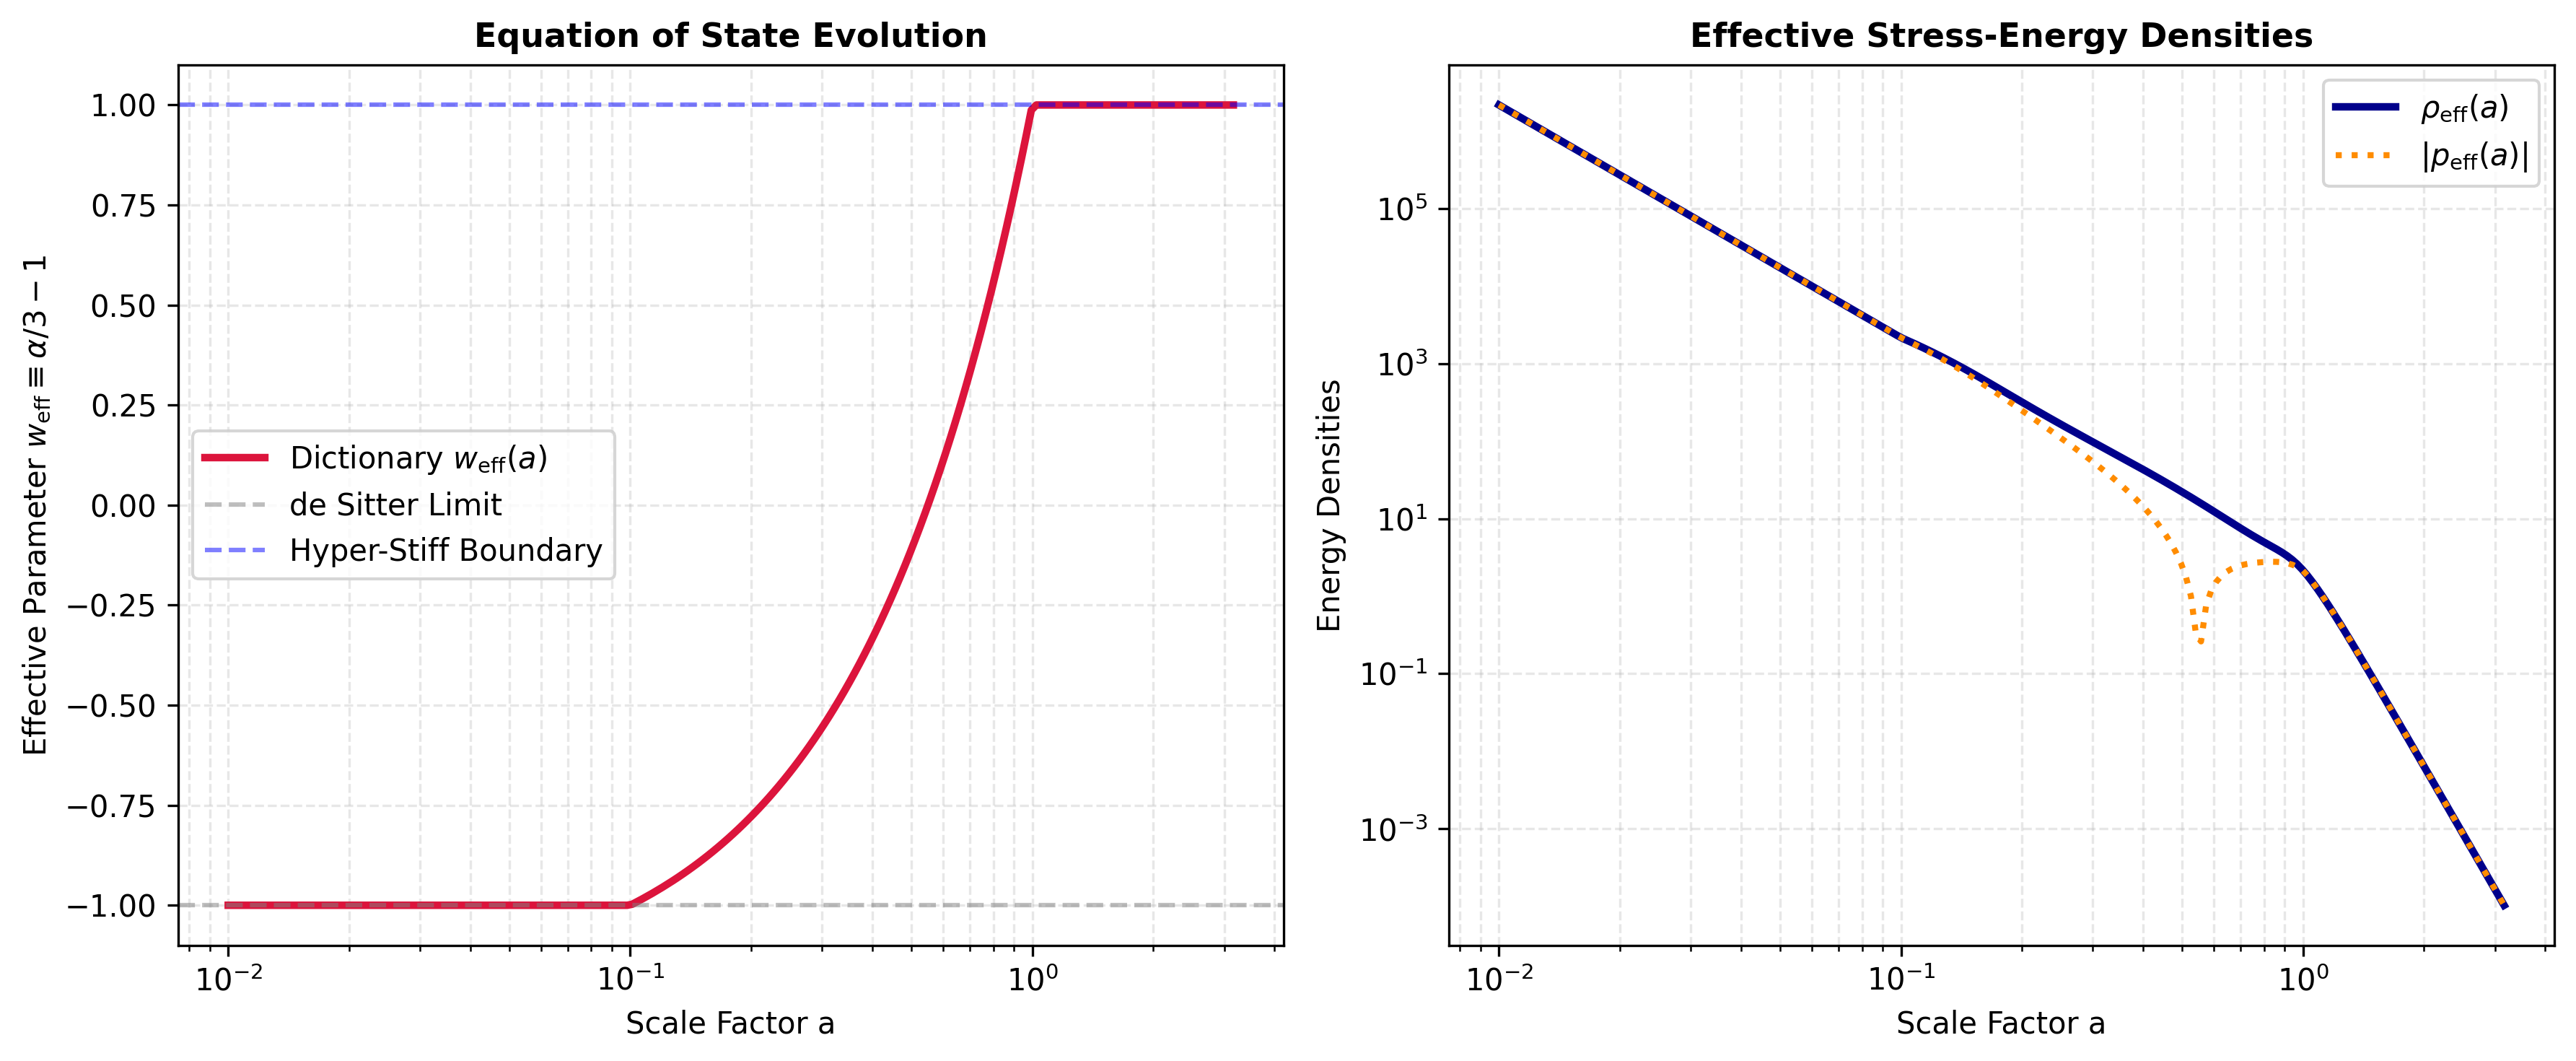
\includegraphics[width=0.95\columnwidth]{figures/stress_energy_tensor_derivation.png}
\caption{\label{fig:stress_energy}
Illustration of the equation-of-state dictionary across an imposed phase schedule $\alpha(a)$ (not
measured or derived; see text).
\textbf{Left Panel:} The macroscopic equation-of-state parameter $w_{\mathrm{eff}}(a)$ obtained by
inserting the imposed schedule $\alpha(a)$ into the dictionary $w_{\mathrm{eff}} = \alpha/3 - 1$. Under
ultraviolet information saturation ($a < 0.1$) the schedule sets $\alpha \to 0$, giving
$w_{\mathrm{eff}} = -1$ by construction; it then sweeps through $\alpha = 3$ (dust, $w = 0$) to $\alpha = 6$
at the causal stiff-matter boundary ($w_{\mathrm{eff}} = 1$).
\textbf{Right Panel:} The corresponding effective energy density $\rho_{\mathrm{eff}}(a)$ and absolute
pressure $|p_{\mathrm{eff}}(a)|$, computed from the same imposed schedule.}
\end{figure}

\section{Conclusion}

We have worked out the effective macroscopic stress--energy tensor implied by a relational quantum
substrate whose mutual information decays as a power law, encoded in the spectrum of the resulting
MI--Laplacian. Given that ansatz, the mapping $T^{\mathrm{eff}}_{\mu\nu}(\mathcal{L}_{\mathrm{MI}})$ follows by
exact algebra and does not depend on the choice of microscopic Hamiltonian generating the
substrate -- but it does depend entirely on the power-law ansatz itself, which we have not derived.

Under the ansatz, the de~Sitter phase appears as the $\alpha \to 0$ limit, where distance
independence pins the cosmic fluid parameter to $w_{\mathrm{eff}} = -1$; a hyper-stiff phase at
$\alpha = 6$ gives $w_{\mathrm{eff}} = 1$. The dictionary $w_{\mathrm{eff}} = \alpha/3 - 1$ links the assumed
entanglement-decay exponent directly to the macroscopic equation of state, offering a candidate
structural link between entanglement geometry and cosmological dynamics -- conditional on that
exponent's evolution being independently justified.

The present work is scoped narrowly: it establishes the algebraic consequences of the power-law MI
ansatz for the effective stress--energy tensor, and nothing more. It does not derive the ansatz
itself; the eigenvalue-ratio check considered in an earlier draft turned out to be circular given
the ansatz's exact homogeneity (Sec.~\ref{sec:scaling}) and provides no independent support for it;
and it does not compare against observational cosmology. All three are open directions, the last of
which is the subject of a planned follow-up analysis.

\end{document}
